\chapter{Wpływ  oddziaływań dalekozasięgowych}
\label{chap:longrange}

\section*{Opis rozdziału}

Ten rozdział bazuje na wynikach opublikowanych w pracy~\cite{wieckowski.ptok.2019}.
Przedstawiona zostanie tutaj analiza dotycząca wpływu oddziaływań dalekozasięgowych na \MZM\ z wykorzystaniem algorytmu wyprowadzonego w rozdziale~\ref{chap:LIOMs}.

\section{Czasy życia modów Majorany}

Jak to przedstawiono w poprzednim rozdziale~\ref{chap:identification}, oddziaływania wielociałowe mają znaczący wpływ na istnienie \MZM\ w  układach oraz na ich rozkład przestrzenny $\alphai$.
Oddziaływania wielociałowe mogą powodować zwiększenie lokalizacji \MZM\ na brzegach układu, jak również mogą powodować zwiększenie zakresu obszaru topologicznego  ze względu na parametry układu, np. ze względu na potencjał chemiczny $\muuniform$.
W tym rozdziale, korzystając z identycznej metody (opisanej w rozdziale~\ref{chap:LIOMs}) jak w rozdziale~\ref{chap:identification} przedstawiono wyniki dotyczące wpływu oddziaływania dalekozasięgowego na \MZM, na przykładzie modelu Kitaeva z oddziaływaniami.
Poszukiwanie \MZM\ w~układach z oddziaływaniami wielociałowymi jest bardzo wymagającym zadaniem.
W przypadku oddziaływań między najbliższymi sąsiadami, w przypadku jednowymiarowych układów, skuteczną metodą jest \acrshort{DMRG}, z pomocą której wpływ tych oddziaływań został już zbadany~\cite{gergs.fritz.2016,thomale.rachel.2013}.
\acrshort{DMRG} umożliwia badanie układów posiadających tysiące węzłów, ale niestety jest zoptymalizowane do badania tylko oddziaływań krótkozasięgowych.
Przedstawiona metoda w rozdziale~\ref{chap:LIOMs} wymaga pełnego spektrum energii, a zatem potrzebna jest metoda bazująca na \acrshort{ED}.
Niestety \acrshort{ED} jest ograniczona do badania bardzo małych układów ($\sites\sim20$)~\cite{kozarzewski.mierzejewski.2019}.
Zasadniczą zaletą metody \acrshort{ED} jest możliwość badania dowolnych oddziaływań: krótkozasięgowych oraz dalekozasięgowych.
Zazwyczaj dodatkowe wyrazy związane z oddziaływaniem typu $\ni\nj$ nie wpływają  na złożoność pamięciową badanych problemów lub ich wpływ jest pomijalnie mały.
W pracy~\cite{wieckowski.ptok.2019} badaliśmy wpływ oddziaływań dalekozasięgowych na czasy życia \MZM\ oraz na ich rozkład przestrzenny.
W tym rozdziale przedstawiono wyniki otrzymane z wykorzystaniem techniki opisanej w rozdziale~\ref{chap:LIOMs} na przykładzie modelu Kitaeva z~oddziaływaniami wielociałowymi dla układu jednowymiarowego drutu z \acrshort{OBC}.
Badany układ może być opisany za pomocą następującego hamiltonianu
\begin{equation}
    \hatH_{\text{Kitaev}+V_r}^{\text{chain}} = 
    \sum_{i=1}^{\sites-1}\left[
    \left(\tuniform \, \aid \aii_{i+1} + \DeltaSCuniform\, \aid \aidii{i+1}\right)
    + \hc\right] -\muuniform \sum_{i=1}^{\sites}  \nz{i}
    +\sum_{r=1}^{\sites-1}\Vuniform_r\sum_{i=1}^{\sites-r}   \nz{i} \nz{i+r}
    ,\label{eq:kitaev+Vr}
\end{equation}
gdzie $\Vuniform_r$ to potencjał oddziaływania pomiędzy $r$-najbliższymi sąsiadami.
Ze względu na to, że dla \acrshort{ED} jest dostępne badanie tylko układów o małych rozmiarach, dla uproszczenia testowano oddziaływania $\Vuniform_r$ do $r=4$.
Rozważano każdy potencjał $\Vuniform_r$ oddzielnie, tzn. dla jednego $r$ ustalano niezerowe $\Vuniform_r$.
W obliczeniach przyjęto $\tuniform=\HBAR=1$.

\begin{figure}
\centering
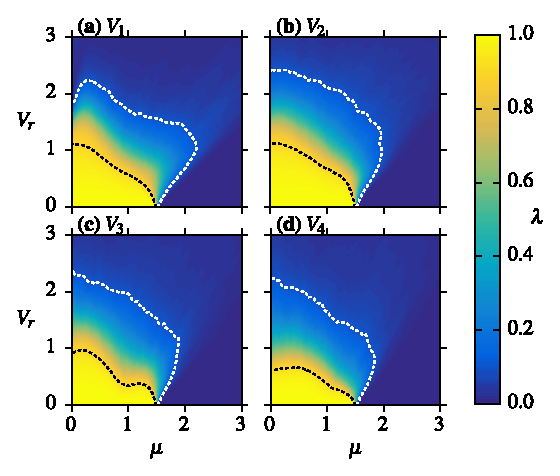
\includegraphics[width=0.8\textwidth]{04-Includes/Figures/LongRange/fig1.pdf}
\caption
[Funkcja autokorelacyjna $\lambda$ w funkcji potencjału chemicznego $\mu$ oraz oddziaływań $V_r$.]
{%
Funkcja autokorelacyjna $\lambdai$ w funkcji potencjału chemicznego $\muuniform$ oraz oddziaływań $\Vuniform_r$.
Wyniki dla $\DeltaSCuniform=0.8$, $\timeTau=50$, $\sites=10$.
Kontrolowane potencjały $\Vuniform_r$ zaznaczono w etykietach wykresu.
Biały i czarny kontur  odpowiada odpowiednio $\lambdai=0.1$ oraz $0.9$.
%
}
\label{fig:VrLambdas1}
%\end{figure}
%\begin{figure}
\centering
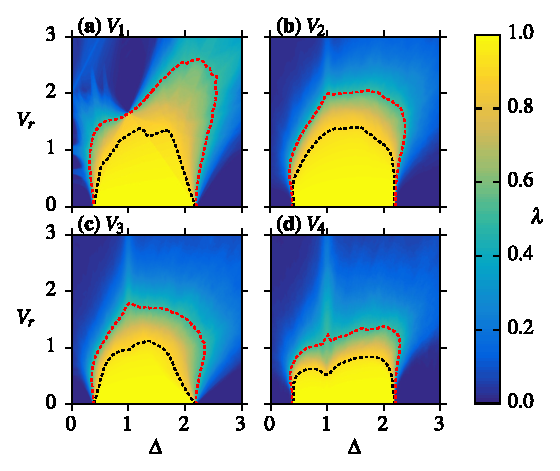
\includegraphics[width=0.8\textwidth]{04-Includes/Figures/LongRange/fig2.pdf}
\caption
[Funkcja autokorelacyjna $\lambda$ w funkcji przerwy nadprzewodzącej $\Delta$ oraz oddziaływań $V_r$.]
{%
Funkcja autokorelacyjna $\lambdai$ w funkcji przerwy nadprzewodzącej $\DeltaSCuniform$ oraz oddziaływań $\Vuniform_r$.
Wyniki dla $\timeTau=50$, $\sites=10$, $\muuniform=0$.
Kontrolowane potencjały $\Vuniform_r$ zaznaczono w etykietach wykresu.
Czerwony i czarny kontur  odpowiada odpowiednio $\lambdai=0.5$ oraz $0.9$.
%
}
\label{fig:VrLambdas2}
\end{figure}

\begin{figure}
\centering
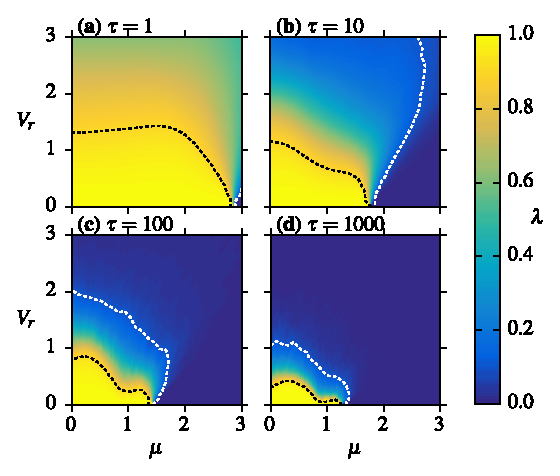
\includegraphics[width=0.8\textwidth]{04-Includes/Figures/LongRange/fig3.pdf}
\caption
[Skalowanie czasowe funkcji autokorelacyjnej $\lambda$ w funkcji potencjału chemicznego $\mu$ oraz oddziaływania $V_3$.]
{%
Skalowanie czasowe funkcji autokorelacyjnej $\lambdai$ w funkcji potencjału chemicznego $\muuniform$ oraz oddziaływania $\Vuniform_3$.
Wyniki dla $\DeltaSCuniform=0.8$, $\sites=10$.
Skale czasowe $\timeTau=10^0,10^1,10^2,10^3$ zaznaczono w etykietach wykresu.
Biały i czarny kontur odpowiada odpowiednio $\lambdai=0.1$ oraz $0.9$.
%
}
\label{fig:VrLambdas3}
%\end{figure}

%\begin{figure}
\centering
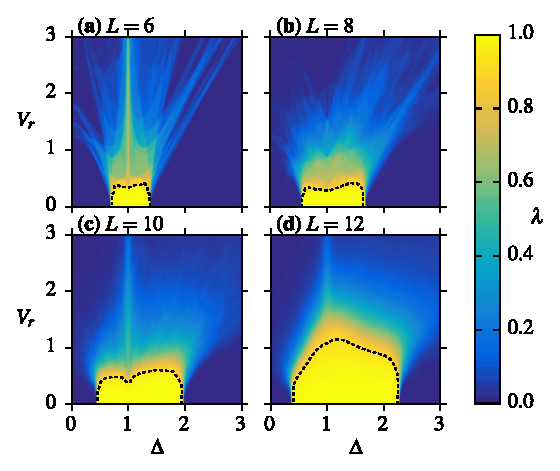
\includegraphics[width=0.8\textwidth]{04-Includes/Figures/LongRange/fig4.pdf}
\caption
[Skalowanie rozmiarowe funkcji autokorelacyjnej $\lambda$ w funkcji przerwy nadprzewodzącej $\Delta$ oraz oddziaływania $V_4$.]
{%
Skalowanie rozmiarowe funkcji autokorelacyjnej $\lambdai$ w funkcji przerwy nadprzewodzącej $\DeltaSCuniform$ oraz oddziaływania $\Vuniform_4$.
Wyniki dla $\timeTau=50$, $\muuniform=0$.
Rozmiary układu $\sites=6,8,10,12$ zaznaczono w etykietach wykresu.
Czarny kontur  odpowiada $\lambdai=0.9$.
%
}
\label{fig:VrLambdas4}
\end{figure}

Na rysunkach \labelcref{fig:VrLambdas1,fig:VrLambdas2,fig:VrLambdas3,fig:VrLambdas4} przedstawiono największą funkcję autokorelacyjną $\lambdai(\timeTau)$.
Analogicznie jak w rozdziale~\ref{chap:identification}, w badanym układzie mogą się znaleźć maksymalnie dwie niezależne \MZM: $\Gammaii^+$ oraz $\Gammaii^-$.
Otrzymane wartości $\lambdai$ dla poszczególnych czasów $\timeTau$ są identyczne dla $\Gammaii^+$ oraz $\Gammaii^-$ --- pokazano wyniki dla jednej z nich.
Znany jest fakt, że $\Vuniform_1$ prowadzi do poszerzenia obszaru topologicznego w potencjale chemicznym $\muuniform$~\cite{stoudenmire.alicea.2011}.
Na rysunku~\ref{fig:VrLambdas1}(a) wyraźnie widać wspomniane zachowanie --- patrz biały kontur.
Takie poszerzenie wydaje się jednak dużo mniejsze dla $\Vuniform_r$, $r>1$ [rysunki~\labelcref{fig:VrLambdas1}(b)--(d)].
Co więcej, obszar gdzie $\lambdai\simeq1$ (strong \MZM) wraz ze wzrostem $r$ zmniejsza się --- porównaj czarny kontur na rysunkach~\ref{fig:VrLambdas1}(a)--(d).
Tak jak napisano w sekcji~\ref{sec:kitaev}, w przypadku braku oddziaływań wielociałowych, $\Vuniform_r=0$, przejście między fazą trywialną a topologiczną dla modelu Kitaeva jest dla $|\muuniform|=2\tuniform$.
Ta ostatnia równość, czyli zależność dla której następuje przejście pomiędzy fazą trywialną, a topologiczną, jest dokładna tylko i wyłącznie w granicy termodynamicznej~\cite{kitaev.2001} --- dla skończonych rozmiarów ta relacja może się różnić.
Na rysunku~\ref{fig:VrLambdas1} to przejście jest dla $|\muuniform|<2\tuniform$.
To jest efekt rozmiarowy i w celu wyznaczenia dokładnej wartości dla wszystkich wyników należałoby dokonać skalowania rozmiarowego i czasowego tak jak w~rozdziale~\ref{chap:identification} [patrz rysunek~\ref{fig:scatteringRatesFSS}].
Taka procedura jest jednak dość skomplikowana i jest obarczona sporym błędem, dlatego w~tym rozdziale taka analiza została pominięta.
Analiza korelacji $\lambdai(\timeTau)$ dla skończonych czasów $\timeTau$ jest wystarczająca do porównania wpływu zasięgu oddziaływania na \MZM.

Na rysunku~\ref{fig:VrLambdas2} przedstawiono analogiczne wyniki jak na rysunku~\ref{fig:VrLambdas1} z tą różnicą, że przedstawiono $\lambdai$ w funkcji potencjałów $\Vuniform_r$ oraz przerwy nadprzewodzącej $\DeltaSCuniform$.
Podobnie wraz ze wzrostem $r$ potencjału $\Vuniform_r$, obszar topologiczny ulega zmniejszeniu [patrz czerwony kontur na rysunku~\ref{fig:VrLambdas2}].
Interesująca jest zanikająca linia wzdłuż wartości $\DeltaSCuniform=1$ na rysunkach~\ref{fig:VrLambdas2}(b)--(d).
Model Kitaeva w punkcie $\DeltaSCuniform=|\tuniform|$ odpowiada szczególnemu przypadkowi parametrów (patrz sekcja~\ref{sec:kitaev})  dla których w przypadku bez oddziaływań, model Kitaeva zawiera \MZM, które są dokładnymi całkami ruchu -- strong \MZM\ ~\cite{kitaev.2001}.
Na rysunku~\ref{fig:VrLambdas2} dla wartości $\DeltaSCuniform\gtrsim2$ w~układzie nie ma \MZM.
Jest to efekt skończonego rozmiaru (analogicznie jak na rysunku~\ref{fig:lambdaResults3} w rozdziale~\ref{chap:identification}), który wyjaśniony będzie na rysunku~\ref{fig:VrLambdas4}.

W celu badania korelacji $\lambdai$ dla układów w granicy termodynamicznej należy zachować szczególną czujność przy kolejności wyznaczanych granic skalowania rozmiarowego i czasowego $\lim_{\sites\to\infty}\lim_{\timeTau\to\infty}$.
W rozdziale~\ref{chap:identification} przedstawiliśmy analizę problemu takiego skalowania.
Jednak w tej części pracy, w celu porównania wpływu zasięgu oddziaływania $r$ potencjału $\Vuniform_r$, analiza związana z wyznaczaniem $\lim_{\sites\to\infty}\lim_{\timeTau\to\infty}\lambdai$ została pominięta.
Przedstawiona została za to analiza jak korelacje $\lambdai$ zależą od $\sites$ oraz $\timeTau$.
Na rysunku~\ref{fig:VrLambdas3} przedstawiono jak $\lambdai$ zależy od potencjału $\Vuniform_3$ oraz potencjału chemicznego $\muuniform$. 
Na poszczególnych rysunkach~\ref{fig:VrLambdas3}(a)--(d) przedstawiono wyniki odpowiednio dla $\tau=10^0,\,10^1,\,10^2,\,10^4$.
Interesujące, że nawet dla bardzo dużego czasu ($\timeTau=1000$), obszar w którym potencjalnie mogą znajdować się \MZM\ jest niezerowy.

Na rysunku~\ref{fig:VrLambdas4} przedstawiono wynik  korelacji $\lambdai$ w funkcji $\Vuniform_4$ oraz $\DeltaSCuniform$.
Na poszczególnych panelach (a)--(d) rysunku~\ref{fig:VrLambdas4} przedstawiono wyniki dla różnych rozmiarów układu, odpowiednio $\sites=6,\,8,\,10,\,12$. 
Na takim zestawieniu wyników widać wyraźne efekty rozmiarowe w korelacji $\lambdai$.
Wraz ze wzrostem rozmiaru układu, obszar (oznaczony kolorem żółtym), gdzie obecna jest faza topologiczna zawierająca strong \MZM, powiększa się.
Takie skalowanie rozmiarowe tłumaczy otrzymany wynik zaprezentowany na rysunku~\ref{fig:VrLambdas2}, gdzie obszar topologiczny np. w przypadku braku oddziaływań wielociałowych ograniczony był do wartości $\DeltaSCuniform\simeq2$.

\ornament

\section{Porównanie z~LUE}

Otrzymane wyniki $\lambdai$ porównano z warunkiem koniecznym istnienia \MZM\ --- degeneracją stanu podstawowego $\deltaE$ [patrz równanie~\eqref{eq:degeneracyFinite}], oraz ze szczeliną energetyczną~ $\DeltaE = \min(\DeltaE_e,\DeltaE_o)$ [patrz równanie~\labelcref{eq:gapFinite1,eq:gapFinite2}], który związany jest z warunkiem równoważności \acrshort{LUE}.
Wyniki dotyczące $\deltaE$ oraz $\DeltaE$ można znaleźć odpowiednio na rysunku~\ref{fig:VrDegeneracy} oraz \ref{fig:VrGap}.
Zaskakujące, że obszar gdzie jest mała degeneracja $\deltaE$, wraz ze wzrostem zasięgu $r$ oddziaływania $\Vuniform_r$ rośnie.
Widoczne linie na rysunku~\ref{fig:VrDegeneracy} nie są związane z istnieniem \MZM, a jedynie z przekrywaniem się poziomów energetycznych [porównaj rysunek~    \ref{fig:degeneracyExplanation}].
Na rysunku~\ref{fig:VrGap} widać, że wraz ze wzrostem $r$, obszar gdzie wartość szczeliny $\DeltaE$ jest duża, rośnie.
Zarówno wyniki dotyczące $\deltaE$ oraz $\DeltaE$ mogą sugerować, że wraz ze wzrostem zasięgu oddziaływania $r$, obszar gdzie mogą występować \MZM rośnie, 
co jest całkowicie odwrotnym zachowaniem w~porównaniu do wyników $\lambdai$ prezentowanych na rysunkach~\labelcref{fig:VrLambdas1,fig:VrLambdas2,fig:VrLambdas3,fig:VrLambdas4}.
Należy tutaj podkreślić, że otrzymane wyniki z algorytmu bazującego na \acrshort{LIOM} oraz wyniki sprawdzonych warunków \acrshort{LUE} nie są ze sobą sprzeczne.
Algorytm bazujący na \acrshort{LIOM} wyznaczył obszary gdzie w układzie mogą być obecne strong \MZM, natomiast warunki \acrshort{LUE} mają informację jedynie o soft \MZM.


\begin{figure}
\centering
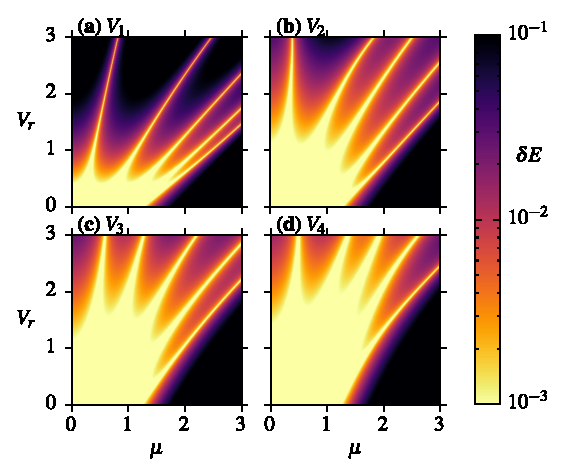
\includegraphics[width=0.8\textwidth]{04-Includes/Figures/LongRange/fig5.pdf}
\caption
[Degeneracja stanu podstawowego $\delta E$ w funkcji $\mu$ oraz $V_r$.]
{
Degeneracja stanu podstawowego $\deltaE$ w funkcji $\muuniform$ oraz $\Vuniform_r$.
Wyniki dla $\DeltaSCuniform=0.8$, $\sites=10$.
}
\label{fig:VrDegeneracy}
\end{figure}

\begin{figure}
\centering
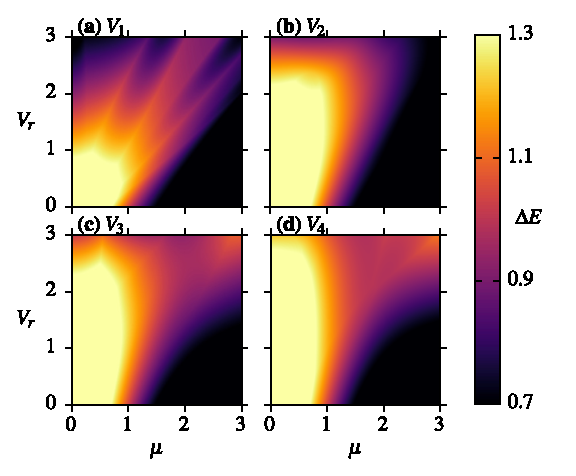
\includegraphics[width=0.8\textwidth]{04-Includes/Figures/LongRange/fig6.pdf}
\caption
[Szczelina energetyczna $\Delta E$ w funkcji $\mu$ oraz $V_r$.]
{
Szczelina energetyczna $\DeltaE$ w funkcji $\muuniform$ oraz $\Vuniform_r$.
Wyniki dla $\DeltaSCuniform=0.8$, $\sites=10$.
}
\label{fig:VrGap}
\end{figure}

\ornament

\section{Wpływ na~strukturę przestrzenną}

W celu wyjaśnienia wyników, zbadano wpływ zasięgu oddziaływania na strukturę przestrzenną \MZM.
Na rysunku~\ref{fig:VrAlpha} zaprezentowano strukturę przestrzenną $|\alphai^+|^2+|\alphai^-|^2$.
Wspomniana wielkość odpowiada znormalizowanej \acrshort{LDOS}~\cite{matsui.sato.2003} lub przewodności różniczkowej~\cite{chevallier.klinovaja.2016}.
Na rysunkach~\ref{fig:VrAlpha}(b)--(d) widać, że wraz ze wzrostem zasięgu $r$ oddziaływania $\Vuniform_r$, lokalizacja \MZM\ zmniejsza się, tzn. suma współczynników $|\alphai^+|^2+|\alphai^-|^2$ na środku łańcucha rośnie, a na brzegach łańcucha maleje.
Dla skończonych układów $\sites\ll\infty$, na skutek przekrywania się \MZM, degeneracja $\deltaE$ jest niezerowa co implikuje skończony czas życia \MZM.
Na rysunku~\ref{fig:VrAlphaAlpha} przedstawiono przekrycie \MZM, które rozumiemy przez $|\alphai^+\alphai^-|$.
Widać tam, że dla środkowych węzłów, przekrycie pomiędzy dwoma \MZM\ rośnie wraz z~zasięgiem $r$ oddziaływania $\Vuniform_r$.

W celu dalszego badania nielokalności \MZM, wykorzystano ich całkowite przekrycie, zdefiniowane następująco~\cite{prada.aguado.2017,deng.vaitiekenas.2018}
\begin{equation}
    \MZMoverlap = \| \Gammaii^+ \widetilde\Gammaii^-\| = \sum_{i=1}^{\sites} |\alphai^+\alphai^-|,
\end{equation}
gdzie $\widetilde\Gammaii^-= U\Gammaii^- U^\dagger$ to odbicie przestrzenne $\Gammaii^+$, a
unitarny operator $U$ opisuje następującą transformację operatorów bazowych
\begin{equation}
    U\gammai^\pm U^\dagger = \gammai^\mp.
\end{equation}
Całkowite przekrycie $\MZMoverlap$, zgodnie z definicją, może przyjmować wartości z przedziału\linebreak $\MZMoverlap\in[0,1]$, gdzie odpowiednio $\MZMoverlap=0$ odpowiada sytuacji kiedy nie ma przekrycia pomiędzy \MZM, a przypadek $\MZMoverlap=1$ odpowiada sytuacji kiedy \MZM przekrywają się całkowicie.
Brak przekrycia, $\MZMoverlap=0$,  jest bezpośrednio wymagany do zapewnienia ochrony topologicznej qubitu bazującego na \MZM\ ~\cite{prada.aguado.2017}.
Należy tutaj podkreślić, że $\MZMoverlap$ jest wielkością, która silnie zależy od rozmiaru układu $\sites$~\cite{dumitrescu.roberts.2015}.



\begin{figure}
\centering
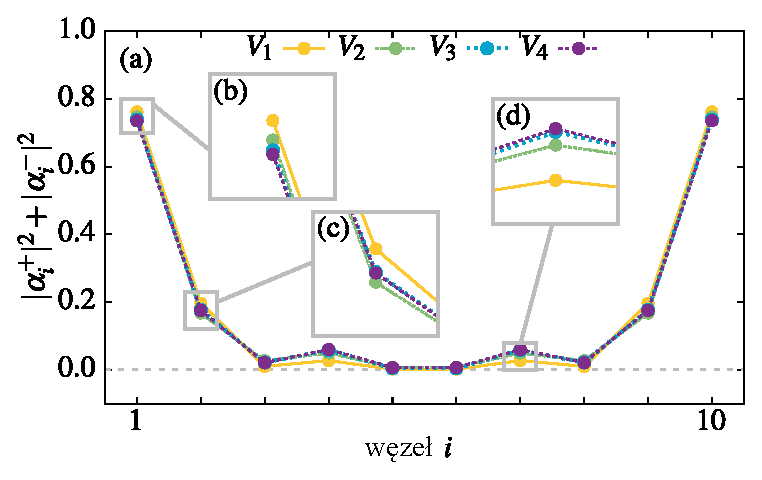
\includegraphics[width=0.7\textwidth]{04-Includes/Figures/LongRange/fig7.pdf}
\caption
[Wpływ zasięgu $r$ oddziaływania $V_r$ na rozkład przestrzenny \textit{MZM}, $\Gamma^+$ oraz $\Gamma^-$.]
{
Wpływ zasięgu $r$ oddziaływania $\Vuniform_r$ na rozkład przestrzenny \MZM, $\Gammaii^+$ oraz $\Gammaii^-$.
Wyniki dla $\sites=10$, $\DeltaSCuniform=0.4$, $\muuniform=0.7$.
}
\label{fig:VrAlpha}
\end{figure}

\begin{figure}
\centering
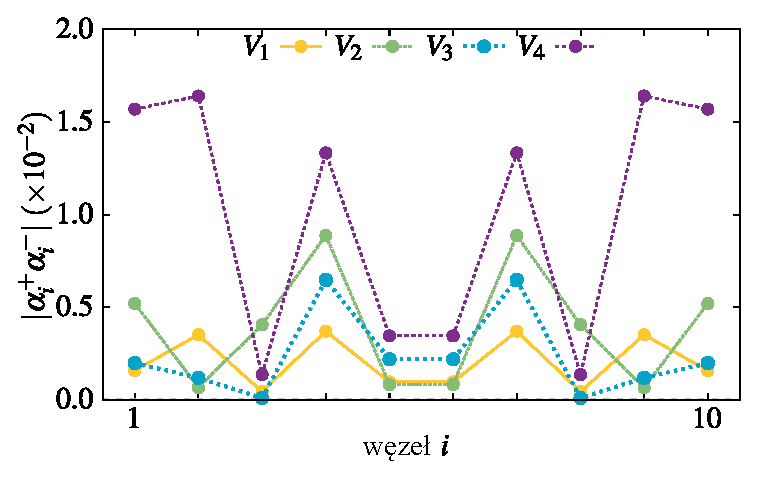
\includegraphics[width=0.7\textwidth]{04-Includes/Figures/LongRange/fig8.pdf}
\caption
[Lokalne przekrycie $|\alpha_i^+\alpha_i^-|$ dla \textit{MZM} $\Gamma^+$ oraz $\Gamma^-$.]
{
Lokalne przekrycie $|\alphai^+\alphai^-|$ dla \MZM\ $\Gammaii^+$ oraz $\Gammaii^-$.
Wyniki dla $\sites=10$, $\DeltaSCuniform=0.4$, $\muuniform=0.7$.
}
\label{fig:VrAlphaAlpha}
\end{figure}

W ogólności całkowite przekrycie $\MZMoverlap$ można kontrolować za pomocą potencjału elektrostatycznego~\cite{ptok.cichy.2018,penaranda.aguado.2018,kobialka.ptok.2019,rainis.trifunovic.2013}, czy też za pomocą oddziaływań międzywęzłowych~\cite{dominguez.cayao.2017,wieckowski.maska.2018}.
W~pracy~\cite{wieckowski.ptok.2019} zbadaliśmy zależność $\MZMoverlap$ od oddziaływań $\Vuniform_r$ oraz potencjału chemicznego $\muuniform$.
Wyniki $\MZMoverlap$ zostały przedstawione na rysunku~\ref{fig:VrOverlap}.
Dla małej wartości oddziaływania $\Vuniform_r$ i potencjału $\muuniform$, całkowite przekrycie $\MZMoverlap$ jest eksponencjalne małe.
Przekrycie $\MZMoverlap$ rośnie wraz ze wzrostem $\Vuniform_r$.
Ten efekt słabo zależy od zasięgu oddziaływania $r$.
Wydaje się, że $\MZMoverlap$ jest bardziej czułe na zmiany potencjału chemicznego $\muuniform$. 
 
Podobne zachowanie można zaobserwować na rysunku~\ref{fig:VrOverlapLocal}, gdzie przedstawiono wyniki numeru węzłów, dla których lokalne przekrycie $|\alphai^+\alphai^-|$ jest największe w funkcji potencjału chemicznego $\muuniform$ oraz oddziaływania $\Vuniform_r$.
Zwiększanie potencjału chemicznego $\muuniform$ powoduje zwiększenie przekrycia \MZM\ na środku łańcucha (w tym wypadku dla $i=5$) -- porównaj z rysunkiem~\ref{fig:VrAlphaAlpha}.
Szybkie zmiany indeksu $i$ w okolicy $\muuniform=1$, związane są z precyzją numeryczną, tzn. wartości $|\alphai^+\alphai^-|$ są relatywnie małe i porównywalne na całej długości łańcucha.
W odróżnieniu od $\muuniform$, oddziaływania $\Vuniform_r$ powodują zwiększenie przekrycia blisko brzegów łańcucha.


\begin{figure}
\centering
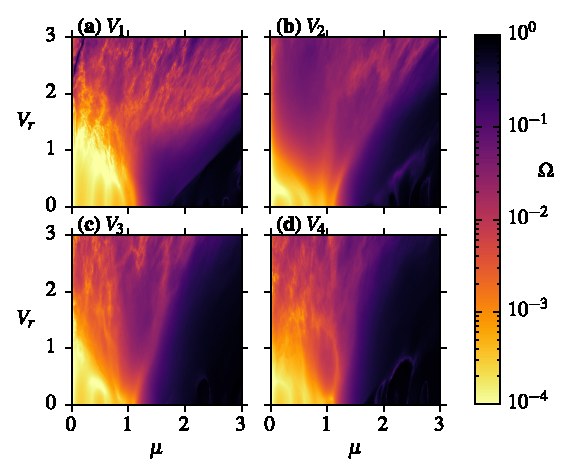
\includegraphics[width=0.8\textwidth]{04-Includes/Figures/LongRange/fig9.pdf}
\caption
[Całkowite przekrycie $\Omega$ pomiędzy \textit{MZM}, $\Gamma^+$ oraz $\Gamma^-$, w funkcji oddziaływań $V_r$ oraz potencjału chemicznego $\mu$.]
{Całkowite przekrycie $\MZMoverlap$ pomiędzy \MZM, $\Gammaii^+$ oraz $\Gammaii^-$, w funkcji oddziaływań $\Vuniform_r$ oraz potencjału chemicznego $\muuniform$.
Panele odpowiadają różnym $\Vuniform_r$, co zaznaczono w etykietach rysunku.
Wyniki dla $\sites=10$, $\DeltaSCuniform=0.8$.
}
\label{fig:VrOverlap}
%\end{figure}
%\begin{figure}
\centering
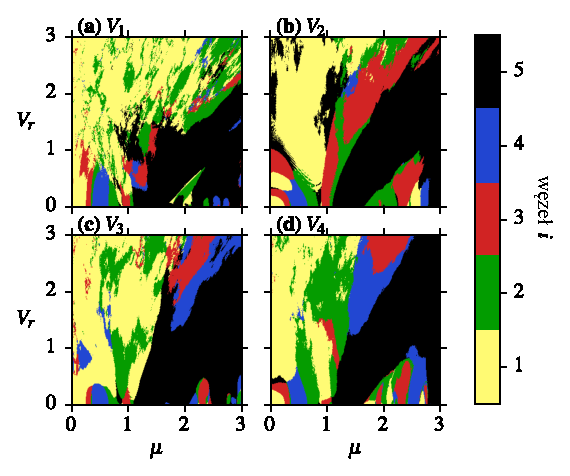
\includegraphics[width=0.8\textwidth]{04-Includes/Figures/LongRange/fig10.pdf}
\caption
[Numer węzła dla którego lokalne przekrycie $|\alpha_i^+\alpha_i^-|$ jest największe, w funkcji oddziaływań $V_r$ oraz potencjału chemicznego $\mu$.]
{
Numer węzła $i$ dla którego lokalne przekrycie $|\alphai^+\alphai^-|$ jest największe, w funkcji oddziaływań $\Vuniform_r$ oraz potencjału chemicznego $\muuniform$.
Panele odpowiadają różnym $\Vuniform_r$, co zaznaczono w etykietach rysunku.
Wyniki dla $\sites=10$, $\DeltaSCuniform=0.8$.
}
\label{fig:VrOverlapLocal}
\end{figure}

\ornament

\section*{Podsumowanie}

Zbadano wpływ zasięgu oddziaływania wielociałowego na czasy życia \MZM\ oraz na ich rozkład przestrzenny.
%Oddziaływania wielociałowe zmniejszają czasy życia \MZM.
Oddziaływania pomiędzy bardziej oddalonymi węzłami są bardziej destrukcyjne od oddziaływań pomiędzy najbliższymi sąsiadami --- w tym pierwszym przypadku, po uwzględnieniu oddziaływań, czasy życia \MZM\ są mniejsze (rysunki~\ref{fig:VrLambdas1}--\ref{fig:VrLambdas2}).
Wraz ze wzrostem zasięgu oddziaływań zmniejsza się lokalizacja \MZM\ na krawędziach układu (rysunek~\ref{fig:VrAlpha}) i równocześnie zwiększa się ich wzajemne przekrywanie (rysunek~\ref{fig:VrAlphaAlpha}).
To zagadnienie dotyczące badania wpływu zasięgu oddziaływania jest szczególnie istotne, ponieważ w prawdziwych materiałach takie oddziaływania są obecne i zanikają wraz z odległością.
Destrukcyjne efekty oddziaływań są również istotne ze względu na zastosowanie \MZM\ w celu przechowywania i przetwarzania informacji kwantowej.
W celu zagwarantowania jak największej efektywności urządzeń bazujących na fizyce \MZM, należało by ograniczać takie oddziaływania tak jak to tylko możliwe.

\ornament



%%%
% Other display to consider

%\begin{figure}
%\hspace{-3cm}
%\begin{minipage}[c]{0.6\textwidth}
%\centering
    %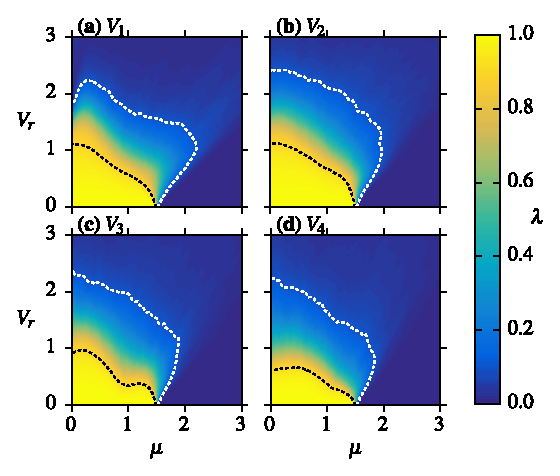
\includegraphics{04-Includes/Figures/LongRange/fig1.pdf}
%    \caption{Caption for image}
    %\label{fig:sample_figure}
%\end{minipage}\hspace{1cm}
%\begin{minipage}[c]{0.6\textwidth}
%\centering
    %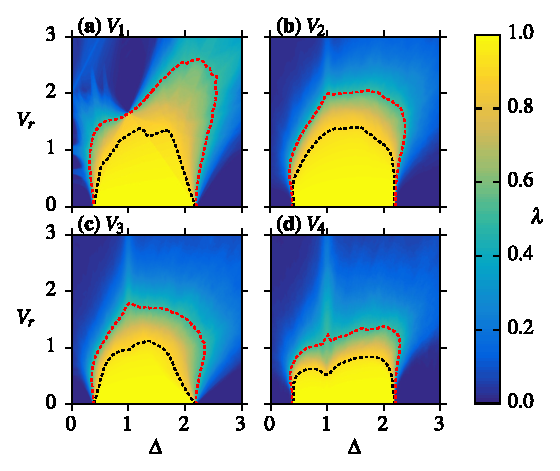
\includegraphics{04-Includes/Figures/LongRange/fig2.pdf}
    %\caption{Caption for image}
    %\label{fig:sample_figure}
%\end{minipage}
%\end{figure}